\renewcommand{\chpath}{2-architecture/}
\renewcommand{\imgpath}{\chpath img/}
\renewcommand{\secpath}{\chpath}
\chapter{Architecture}
\label{chap:archi}

\newcommand{\imgW}{.8}

Dans cette partie, nous présentons l'architecture du projet, et détaillons en particulier la reconstruction de modèles. AngioTK prend la forme d'une chaîne de traitement (on parle de pipeline logiciel) qui prend une image IRM de cerveau en entrée et lui fait traverser une succession d'étapes menant à la simulation d'IRM. Chacune de ces étapes correspond à un logiciel à part entière (ou brique logicielle) inséré dans la chaîne.

\section{Images IRM à traiter}

Afin de pouvoir mettre au point et tester le pipeline, plusieurs images IRM ont été utilisées. Elles sont regroupées dans 3 bases de données.

\subsection{Base 1}

La base 1 contient 71 IRM...

\subsection{Base 2}

La base 2 contient 38 IRM acquises dans le cadre du projet. La taille des voxels est $0,8\times0,8\times0,8$ \SI{}{\milli\meter\cubed}

\subsection{Base 3}

La base 3 rassemble les IRM de 94 patients. Ces données proviennent de la base de donnée publiée par Elizabeth Bullitt (\href{http://www.insight-journal.org/midas/community/view/21}{http://www.insight-journal.org/midas/community/view/21}). Les angiographies ont été acquises avec des voxels de $0,5\times0,5\times0,8$ \SI{}{\milli\meter\cubed}.

%\newpage

\section{Pipeline de reconstruction de modèle}

\subsection{Principe général}

La reconstruction de modèle 3D et la génération de maillage ont lieu en plusieurs étapes. L'organisation de ces étapes suit le schéma général suivant:

\ 

On part d'une image 3D (IRM), on isole les structures d'intérêt (les vaisseaux sanguins) dans cette image 3D et on extrait leur surface. Enfin, on en génère un maillage du volume correspondant.

\ 

Cependant, des étapes intermédiaires sont nécessaires afin d'obtenir un résultat acceptable en vue des simulations. Dans la suite, le détail de l'architecture du pipeline permet de comprendre pourquoi.

\ 

\subsection{Filtrage des images}

L'isolation des structures d'intérêt est assurée par le logiciel \rorpo. Il filtre les images 3D pour mettre en valeur les structures tubulaires qu'elles contiennent.

\begin{figure}[H]
\begin{center}
  \subfigure[]{ \includegraphics[width=.8\linewidth]{\imgpath 0_mri}\label{fig:0mri}}
  \subfigure[]{ \includegraphics[width=.8\linewidth]{\imgpath 1_rorpo}\label{fig:1rorpo}}
\caption{Image IRM avant \subref{fig:0mri} et après filtrage \subref{fig:1rorpo}.
}
\end{center}
\label{fig:rorpo}
\end{figure}

\subsection{Extraction de surface}

À partir de l'image filtrée, on peut extraire la surface des vaisseaux sanguins. Cependant, on obtient une surface très irrégulière (c'est une conséquence du bruit présent à l'origine dans l'image). C'est pourquoi on ne passe pas directement à la génération de maillage.

\begin{figure}[H]
\begin{center}
  \subfigure{ \includegraphics[width=\imgW \linewidth]{\imgpath 2_sfi}\label{fig:2sfi}}
\caption{Surface extraite.% \subref{fig:2sfi}.
}
\end{center}
\label{fig:sfi}
\end{figure}

\subsection{Définition des lignes centrales}

L'idée actuellement implantée consiste à se servir de ce modèle imparfait pour trouver et extraire les lignes centrales des vaisseaux sanguins. L'idée est ensuite de s'en servir pour reconstruire un modèle plus régulier et débarrassé du bruit.

\begin{figure}[H]
\begin{center}
  \subfigure{ \includegraphics[width=\imgW \linewidth]{\imgpath 3_cl}}%\label{fig:3cl}}
\caption{Lignes centrales d'une partie du modèle.% \subref{fig:3cl}.
}
\end{center}
\label{fig:cl}
\end{figure}

\subsection{Génération d'une nouvelle image 3D}

Ces lignes centrales servent d'abord à créer une image 3D (semblable à l'IRM de départ). Cette image de synthèse ne contiendra que des vaisseaux sanguins reconstruits à partir des lignes centrales. Les avantages sont l'absence de bruit et la régularité obtenue.

\begin{figure}[H]
\begin{center}
  \subfigure{ \includegraphics[width=\imgW \linewidth]{\imgpath 4_ifcl}}%\label{fig:4ifcl}}
\caption{Image générée à partir des lignes centrales.% \subref{fig:4ifcl}.
}
\end{center}
\label{fig:ifcl}
\end{figure}

\subsection{Deuxième extraction de surface}
\label{arch:sfi2}

Une deuxième extraction de surface, en utilisant l'image 3D générée, permet alors d'obtenir un modèle 3D très régulier.

\begin{figure}[H]
\begin{center}
  \subfigure{ \includegraphics[width=\imgW \linewidth]{\imgpath 5_sfi2}}%\label{fig:5sfi2}}
\caption{Surface extraite.% \subref{fig:5sfi2}.
}
\end{center}
\label{fig:sfi2}
\end{figure}

\subsection{Traitement de surface}

On remaille la surface et on ouvre les extrémités des vaisseaux sanguins.

\begin{figure}[H]
\begin{center}
  \subfigure{ \includegraphics[width=\imgW \linewidth]{\imgpath 6_sm}}%\label{fig:6sm}}
\caption{Maillage surfacique avec extrémités ouvertes.% \subref{fig:6sm}.
}
\end{center}
\label{fig:vm}
\end{figure}

\subsection{Génération de maillage volumique}
\label{arch:vm}

On remaille le volume et on génère un fichier de description pour les simulations. On peut également extruder une couche d'épaisseur pour la paroi des vaisseaux sanguins.

\begin{figure}[H]
\begin{center}
  \subfigure{ \includegraphics[width=\imgW \linewidth]{\imgpath 7_vm}}%\label{fig:7vm}}
\caption{Maillage volumique.% \subref{fig:7vm}.
}
\end{center}
\label{fig:vm}
\end{figure}

\newcommand{\figpart}{.5}
\newcommand{\hpart}{1.}

\begin{center}
 \begin{figure}[H]
	\begin{minipage}[t]{\figpart \linewidth}
            	\centering
            	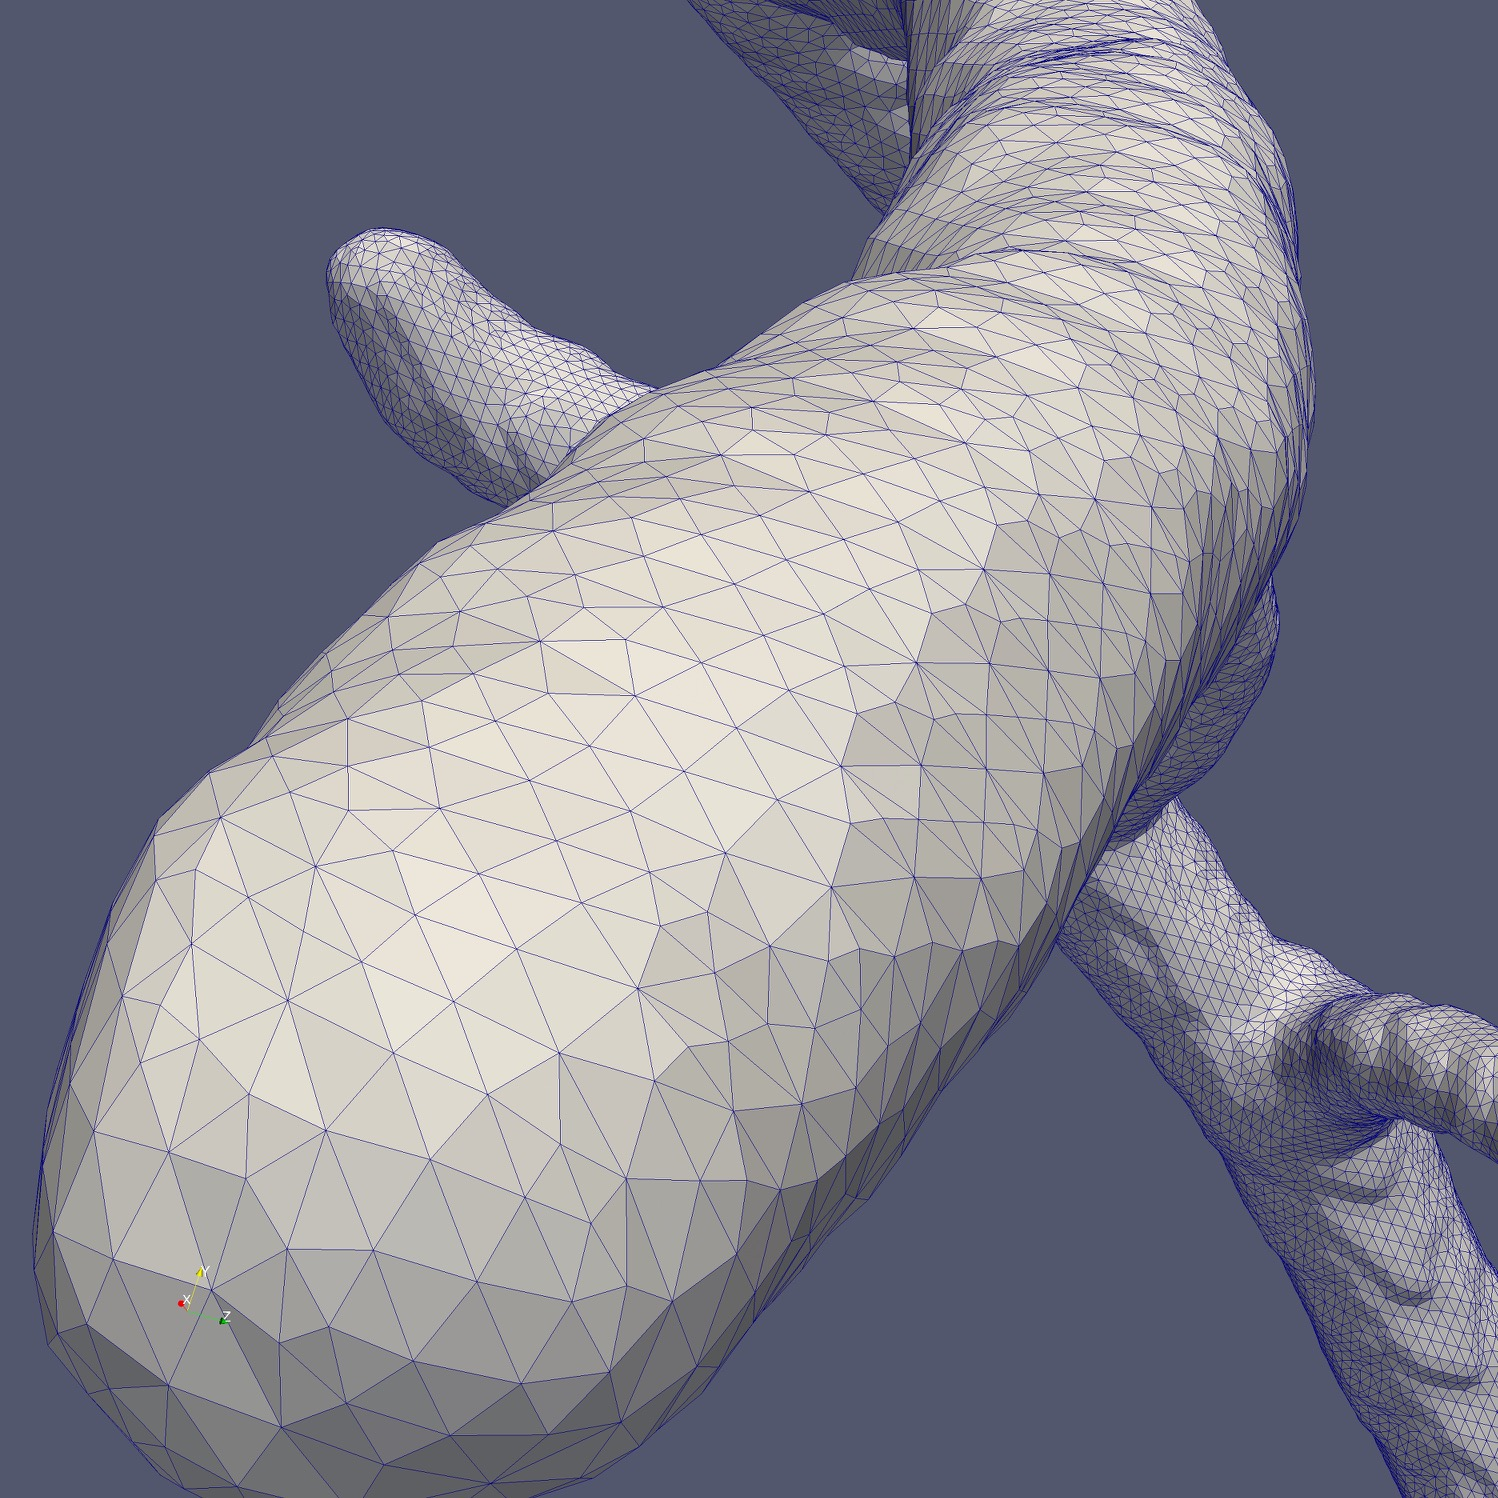
\includegraphics[width=\linewidth,height=\hpart \textheight,keepaspectratio]{\imgpath alt/cu/5_sfi2_wf_cu2}
		\caption*{Surface extraite}
	\end{minipage}
	\begin{minipage}[t]{\figpart \linewidth}
            	\centering
            	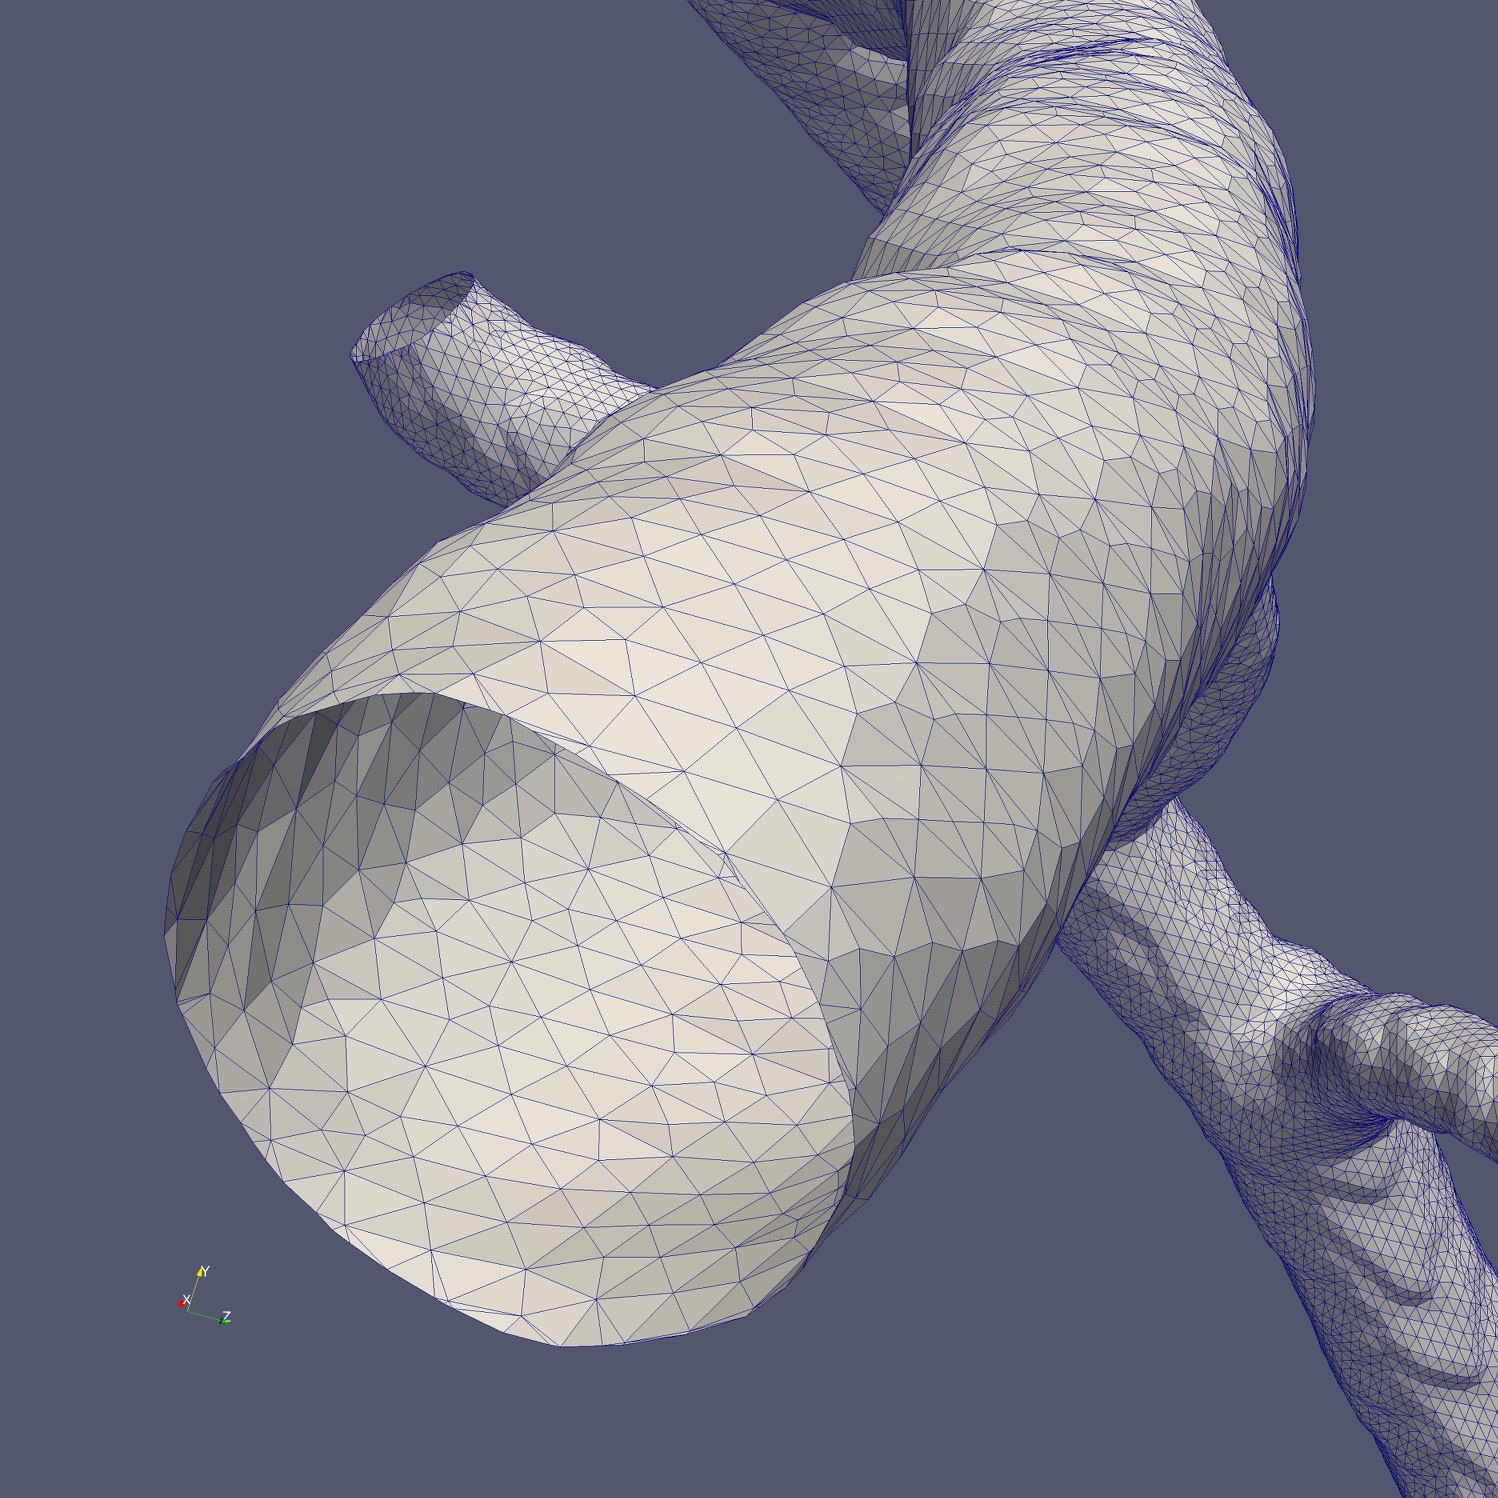
\includegraphics[width=\linewidth,height=\hpart \textheight,keepaspectratio]{\imgpath alt/cu/6_sm_open_wf_cu2}
		\caption*{Ouverture}
	\end{minipage}
	\begin{minipage}[t]{\figpart \linewidth}
            	\centering
            	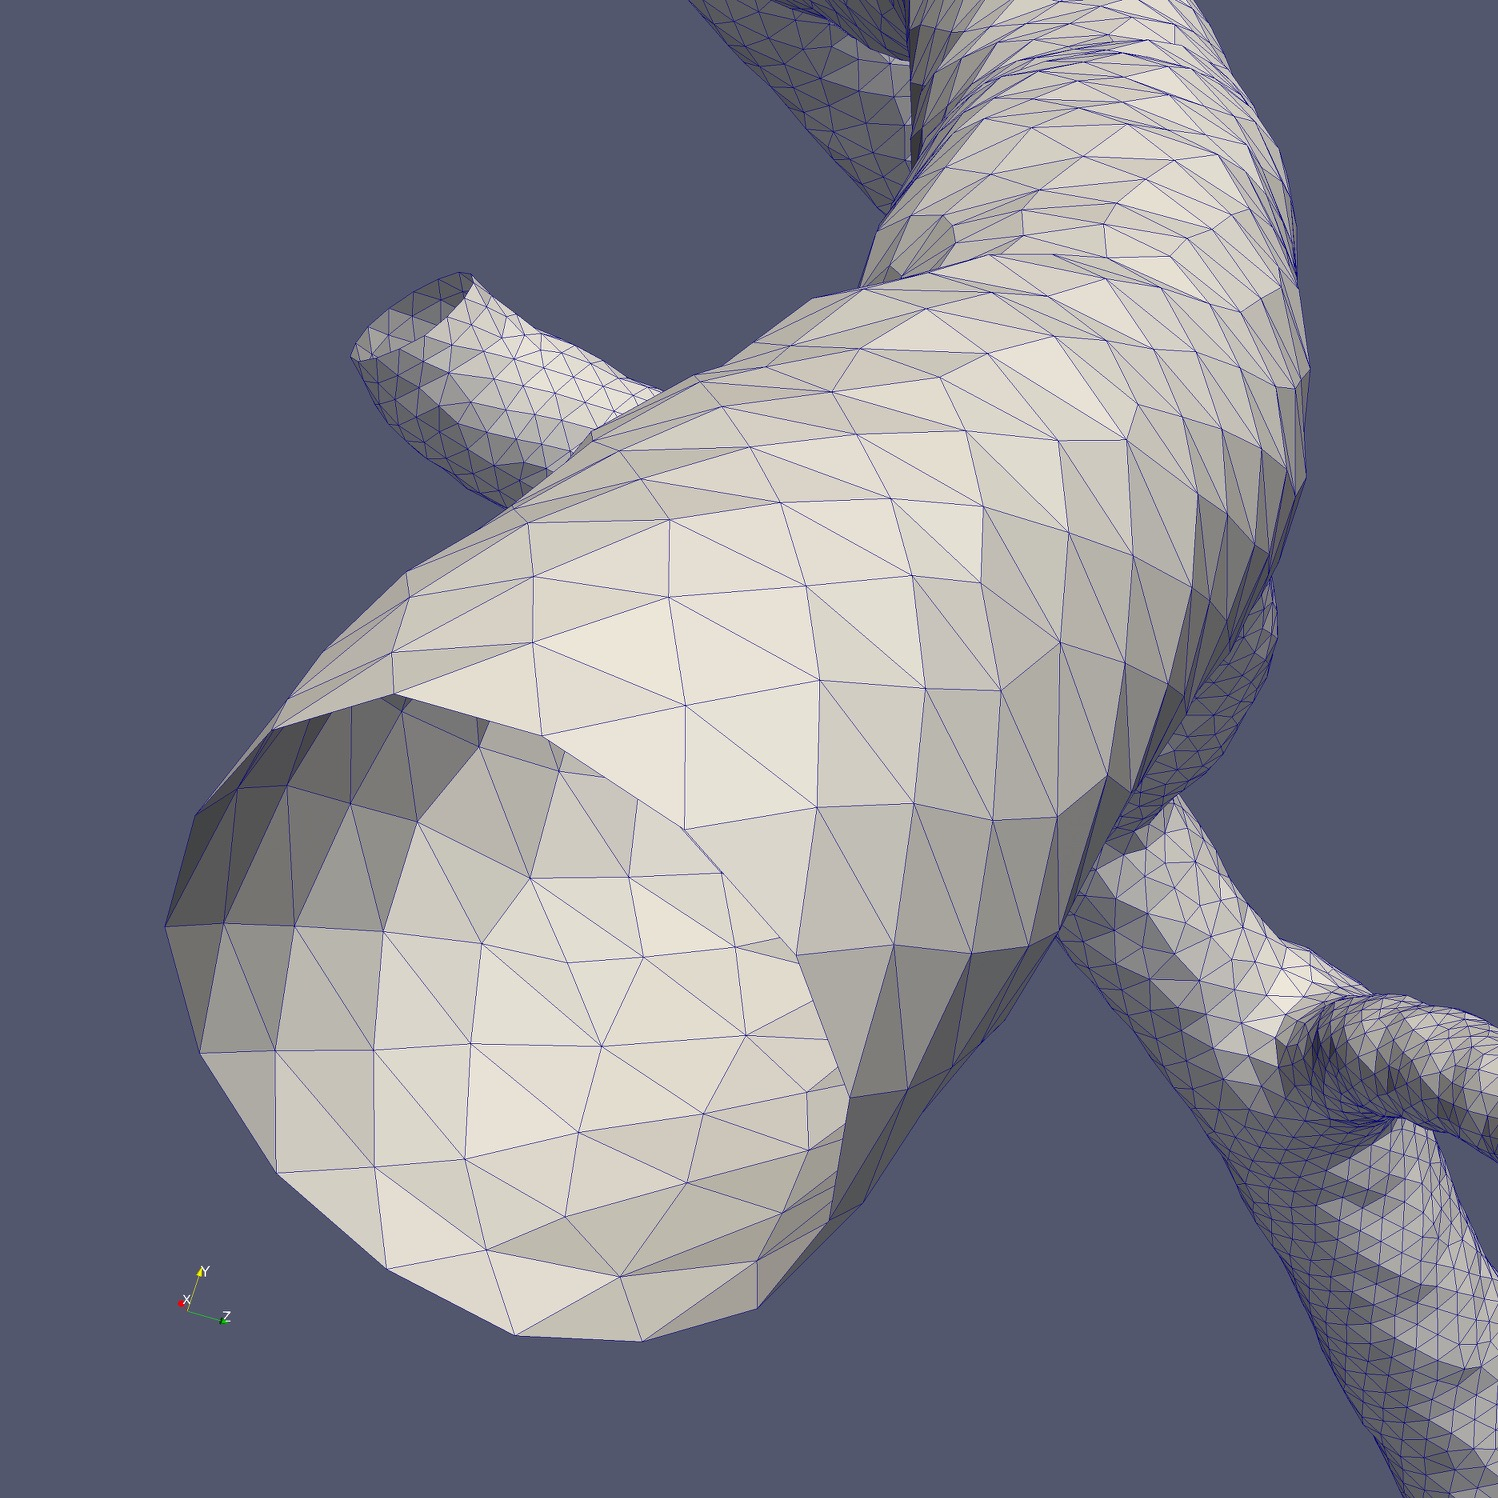
\includegraphics[width=\linewidth,height=\hpart \textheight,keepaspectratio]{\imgpath alt/cu/6_sm_remesh_wf_cu2}
		\caption*{Remaillage surfacique}
	\end{minipage}
	\begin{minipage}[t]{\figpart \linewidth}
            	\centering
            	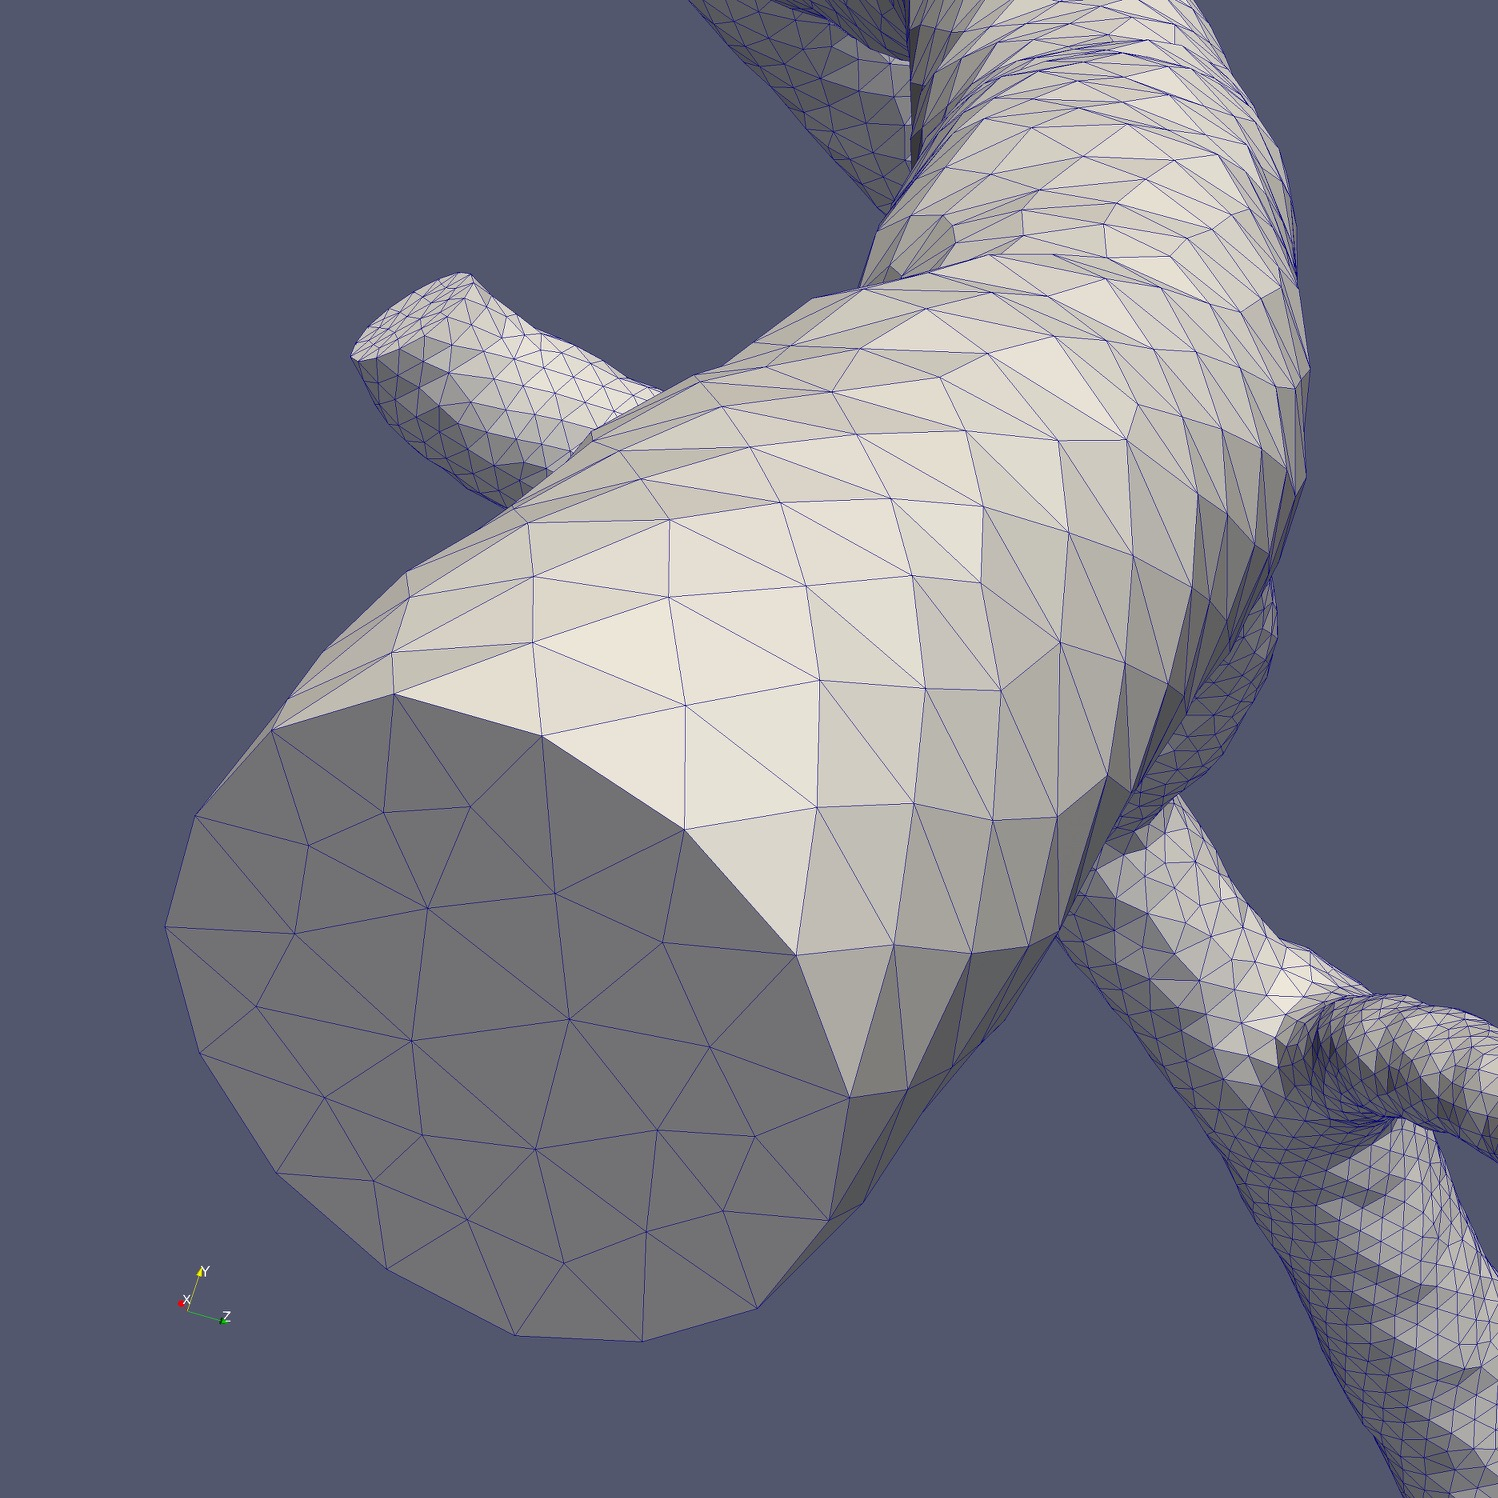
\includegraphics[width=\linewidth,height=\hpart \textheight,keepaspectratio]{\imgpath alt/cu/7_vm_wf_cu2}
		\caption*{Maillage volumique}
	\end{minipage}
	
	\caption{Evolution d'une extrémité de vaisseau sanguin au cours des étapes \ref{arch:sfi2} (\nameref{arch:sfi2}) à \ref{arch:vm} (\nameref{arch:vm}).}
 \end{figure}
\end{center}

\section{Simulation d'écoulements (Feel++)}

Disposant d'un maillage adapté des vaisseaux sanguins, nous pouvons y réaliser des simulations d'écoulements. Ces simulations sont réalisées grâce à Feel++...

\section{Simulation d'angiographies virtuelles (JEMRIS)}

Il est également possible de simuler des IRM de ces modèles reconstruits, afin de réaliser des angiographies virtuelles. Ces simulations sont réalisées grâce à JEMRIS...

